\chapter{基于PCDM的极化SAR图像舰船目标检测}
\label{cha:PCDM}

\section{引言}
\label{sec:chap4:sec1}
在第\ref{cha:PWF}章与第\ref{cha:LMM}章,我们实现了基于PWF与LMM模型的舰船检测算法,这两种方法都是
对图像强度信息进行统计建模以区分舰船目标与背景杂波。然而基于强度或幅值的统计方法易受海况的影响导致
对海杂波的拟合程度不够精确,使得检测性能下降。在本章中我们实现了基于极化协方差差异矩阵的极化SAR
舰船目标检测方法。在极化SAR图像中,舰船目标点的邻域像素提供了丰富的空间相干信息,极化协方
差矩阵主要度量了待检测像素与其3\times 3邻域像素的协方差矩阵的差异。基于该极化差异矩阵,我们首先应用SPAN检测器得到了
粗略的舰船检测结果。同时我们将PCDM矩阵进行极化分解提取了新的极化特征基础船高(PSH),通过此极化特征结合SPAN检测器
给出的初步检测结果进行综合判断得到最终的舰船检测结果。




\section{PCDM理论背景}
\label{sec:chap4:sec2}
\subsection{极化SAR散射表征与SPAN理论}
    通常散射矩阵被用来描述目标散射体的极化信息。在使用水平与垂直极化基的典型极化SAR系统中,复散射矩阵
    定义为如下的形式~\cite{book},其中$S_{HH}$代表了水平发射水平接收的极化信息,当满足互易性的条件时,$S_{HV}=S_{VH}$此时复散射
    矩阵可用三维的复散射矢量$k$表示,如式\ref{equ:chap4:kvector}所示。

    \begin{equation}
        \label{equ:chap4:Smatrix}
        S = \left[ {\begin{array}{*{20}{c}}
        {{S_{HH}}}&{{S_{HV}}}\\
        {{S_{VH}}}&{{S_{VV}}}
        \end{array}} \right]
    \end{equation}

    \begin{equation}
        \label{equ:chap4:kvector}
        k = [{S_{HH}},\sqrt 2 {S_{HV}},{S_{VV}}]
    \end{equation}

    将散射矩阵进行变换可以得到更多散射体的极化信息,式\ref{equ:chap4:cov}为散射矢量对应的极化协方差矩阵~\cite{Zhang2018Ship}。在该式
    中$\left\langle {} \right\rangle$代表在空间域上求平均,$\left| {} \right|$代表幅度值,$H$代表共轭转置。

    \begin{equation}
        \label{equ:chap4:cov}
        [C] = \left\langle {k \cdot {k^H}} \right\rangle  = \left[ {\begin{array}{*{20}{c}}
        {{C_{11}}}&{{C_{12}}}&{{C_{13}}}\\
        {{C_{21}}}&{{C_{22}}}&{{C_{23}}}\\
        {{C_{31}}}&{{C_{32}}}&{{C_{33}}}
        \end{array}} \right]
    \end{equation}

    在极化协方差矩阵$C$中,将对角线元素之和定义为为后向散射总功率即SPAN,如式\ref{equ:chap4:span}所示。还可以对
    极化协方差矩阵进行分解如式\ref{equ:chap4:decompose}所示~\cite{Liu2010Statistical},其中$\lambda_i$为极化协方差矩阵特征值,$v_i$为$\lambda_i$对应的
    特征向量。
    \begin{equation}
        \label{equ:chap4:span}
        {\rm{SPAN}} = {C_{11}} + {C_{22}} + {C_{33}}
    \end{equation}
    \begin{equation}
        \label{equ:chap4:decompose}
      C = \sum\limits_{i = 1}^3 {{\lambda _i}({v_i} \cdot {v_i}^H)} 
    \end{equation}

    \subsection{极化协方差差异矩阵}
    在计算机视觉领域,LBP特征(局部二值模式)用来描述光学图像中的纹理特征,被广泛应用于人脸检测与目标识别。
    LBP特征是将一个3\times 3区域内的中心像素值与邻域像素值做比较,并将得到的八位二进制结果重新排列构成一新二进制数值,
    该数值作为此区域中心像素的LBP特征值,如式\ref{equ:chap4:LBP}所示,其中$g_i$表示邻域内第i个像素的灰度值,
    $g_c$为中心像素灰度值,$x_c, y_c$表示中心像素坐标。

    \begin{equation}
        \label{equ:chap4:LBP}
        [LB{P_{({x_c},{y_c})}} = \sum\limits_{i = 0}^{n - 1} {{2^{is({g_i} - {g_c})}}} ,s(x) = \left\{ {\begin{array}{*{20}{c}}
        1&{x \ge 0}\\
        0&{x < 0}
        \end{array}} \right.
    \end{equation}

    类比光学图像中的LBP特征~\cite{Lan2017Quaternionic},在极化SAR图像中,采用极化协方差矩阵来描述图像的极化信息。在光学图像中像素的灰度值
    可以通过R、G和B三个通道进行计算得到,而极化协方差矩阵也包含了极化SAR图像的HH、HV和VV通道的信息,但区别是灰度值
    只含有图像的一个特征,而极化协方差矩阵包含了九个极化特征,因此对LBP模型进行改进引入极化协方差差异矩阵(PCDM)

    定义${C^{(x,y)}}$为极化SAR图像索引为$x,y$像素处的极化协方差矩阵,接下来计算其3\times 3邻域上的协方差矩阵累积差异$P^{(x,y)}$,
    称$P^{(x,y)}$为极化SAR图像$x,y$处的极化协方差差异矩阵~\cite{张程2018基于},如式\ref{equ:chap4:PCDM}所示,其中$C_{m,n}^{(i,j)}$为
    图像索引$(i,j)$处协方差矩阵的第$(m,n)$个元素。

    \begin{equation}
        \label{equ:chap4:PCDM}
        P_{m,n}^{(i,j)} = \sum\limits_{\Delta i =  - 1,\Delta j =  - 1}^1 {\left| {C_{m,n}^{(i,j)} - C_{m,n}^{(i + \Delta i,j + \Delta j)}} \right|}
    \end{equation}

    \begin{figure}[H] % use float package if you want it here
      \centering
      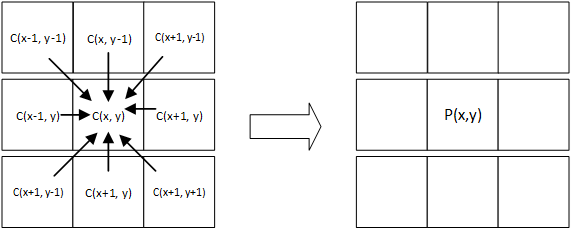
\includegraphics[width=0.9\textwidth]{PCDMCal.png}
      \caption{PCDM矩阵计算示意图}
      \label{fig:chap4:PCDM}
    \end{figure}   
  \section{基于PCDM的舰船目标检测算法}
      前三节我们描述了PCDM可以综合利用待检测像素与其邻域的像素的相干信息,在此基础上我们
      提出了基于极化协方差差异矩阵的舰船检测方法。对于输入的原始极化SAR图像数据,我们首先计算
      每个像素的极化协方差矩阵,然后按照式\ref{equ:chap4:PCDM}计算每个像素对应的极化协方差差异
      矩阵。得到极化协方差差异矩阵$\bf{P}$后,首先对$\bf{P}$矩阵应用SPAN检测器,即当$\rm{SPAN}_{\bf{P}}$>$T_{\rm{SPAN}}$
      时,认定该检测像素为舰船目标像素。

      对PCDM矩阵应用SPAN检测器后输出初步检测结果,为了提升检测的精度,我们进一步提取极化
      协方差差异矩阵的极化特征来区分舰船目标与背景杂波。通常SAR图像目标散射特性可以用极化特征来描述,例如
      极化分解,极化反对称性等极化特征。在文献~\cite{Durden1990The}中提出了pedestal height特征来描述目标的散射特性,
      该极化特征实质上等价于极化协方差矩阵最小特征值与最大特征值的比值。实验表明低海况的背景杂波与方位向模糊像素的
      pedestal height极化特征值比真实的舰船像素要低很多。
       \begin{equation}
          {\rm{PSH = }}\frac{{\left| {{\lambda _3}} \right|}}{{\left| {{\lambda _1}} \right| + \left| {{\lambda _2}} \right|}}
      \end{equation}

      基于极化协方差差异矩阵我们重新计算这些极化特征,并将第二特征值考虑在内,新的极化特征命名为pedestal ship height(PSH)。对于提取的PSH极化特征,应用适当
      的检测阈值,来区分舰船目标与背景杂波像素。整个算法的流程如图\ref{fig:chap4:PCDMalg}所示,算法描述如算法\ref{alg:chap4:PCDMALG}所示

    \begin{figure}[H] % use float package if you want it here
      \centering
      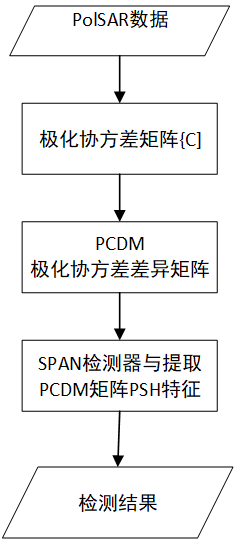
\includegraphics[height=0.5\textwidth]{PCDMalg.png}
      \caption{PCDM检测流程示意图}
      \label{fig:chap4:PCDMalg}
    \end{figure}

    \begin{algorithm}[t]
      \caption{基于PCDM的舰船检测算法}
      \label{alg:chap4:PCDMALG}
      \KwIn{原始极化SAR图像数据}
      \BlankLine
      初始化,计算每个像素的协方差矩阵。

      \ForEach{图像中的像素}{
          根据协方差矩阵计算该像素对应的极化协方差差异矩阵

          计算该极化协方差差异矩阵的SPAN值

          计算极化协方差差异矩阵的基础船高(PSH)极化特征

          将差异矩阵SPAN值与经验阈值作比较,如果$\rm{SPAN}_{PCDM}>T_{SPAN}$,则将该像素为舰船像素。

          将极化特征PSH与经验阈值作比较,如果$PSH_{P(x,y)}>T_{PSH}$,则该像素为舰船像素

      }
      \KwOut{最终舰船检测结果$result$}  
    \end{algorithm}

\section{基于GPU的PCDM算法设计}
      
      前几节描述了基于极化协方差差异矩阵的舰船目标检测算法,在该方法中需要对计算SAR图像每一个像素对应的协方差差异矩阵
      与其极化特征PSH。在该方法中不同像素对应的极化协方差差异矩阵不同,且极化特征估计相互独立,因此将对每个像素的检测
      操作一一对应到GPU上的每个线程。

      线程模块大小设计,本次实验的原始SAR图像数据大小为1000x1000,线程块中的线程以32个为一组进行调度,为充分利用流多处理器
      资源,将线程块大小设计为32x32。考虑到GPU同时并发线程数量的限制与全局内存空间容量,将线程网格大小设计为16x16,对于线程块中的线程
      通过其二维线程索引(threadIDx)与原始SAR图像上的列一一对应,使用线程块索引(blockIDx)与原始SAR图像的行去对应。
      我们设计的线程网格数量为256小于原始SAR图像的行数,因此对SAR图像的检测操作将被分配到四个内核中去执行。内核中的线程通过
      内核序号来找到自己对应的SAR图像行索引,四个内核被装载到同一CUDA流中在GPU上被顺序调度。线程内存空间设计,在CUDA架构中
      不能在核函数中去动态声明较大的内存区域,因此需要在内核执行前由主机分配好线程内存池,然后线程根据自身索引与给定的线程空间大小去找到
      本线程私有内存空间的起始地址。线程内存空间分析,对于PCDM方法,要存储九个像元的散射矩阵信息、协方差矩阵信息与中心像元的极化协方差
      差异矩阵,综合考虑PCDM矩阵计算特征值等其他计算开销,最终我们一个线程所占有的内存空间设置为8192B。

      内核函数的设计,首先计算本线程所对应的二维索引,将该二维索引与其3x3邻域对应的SAR图像数据从全局内存复制到
      线程私有的内存空间中,之后计算这九个像元所对应的协方差矩阵并调整为9x9大小,该矩阵每一列代表各像元的协方差
      矩阵元素。将该矩阵的第五列即中心像素的协方差矩阵与其他列依次做差求绝对和得到极化协方差差异矩阵。得到PCDM矩阵后,首先对
      该矩阵应用SPAN检测器,即计算矩阵对角线元素之和并与经验阈值做比较,当该SPAN值大于经验阈值时,将该像素判别为舰船像素。
      接下来计算极化协方差差异矩阵的PSH极化特征,该特征为PCDM矩阵最小特征值与其他两个特征值绝对值之比,因此问题转化为
      计算极化协方差差异矩阵特征值的问题。PCDM矩阵为实对称矩阵,计算其特征值采用雅克比迭代的方式,迭代过程的矩阵更新
      公式如式\ref{equ:chap4:jacobian}所示,其中$\varphi$通过选择矩阵非对角绝对值最大元素计算得到。具体的算法流程为
      算法\ref{alg:chap4:jacobianeigen}所示。得到矩阵的特征值后计算PSH极化特征的大小并与经验阈值做比较,如果PSH值大于
      经验阈值,则判断该像素为舰船目标像素。当GPU上所有线程核函数执行结束后,主机将检测结果从设备内存拷贝至主机内存,结合
      OpenCV进行图像显示,并保存检测结果。

       \begin{equation}
           \label{equ:chap4:jacobian}
            \begin{array}{*{20}{c}}
            {\left\{ {\begin{array}{*{20}{c}}
            {a_{pp}^{i + 1} = a_{pp}^i{{\cos }^2}\varphi  + a_{qq}^i{{\sin }^2}\varphi  + 2a_{pq}^i\cos \varphi \sin \varphi }\\
            {a_{qq}^{i + 1} = a_{pp}^i{{\cos }^2}\varphi  + a_{qq}^i{{\sin }^2}\varphi  - 2a_{pq}^i\cos \varphi \sin \varphi }\\
            {a_{pq}^{i + 1} = a_{qp}^{i + 1} = \frac{1}{2}(a_{qq}^i - a_{pp}^i)\sin 2\varphi  + a_{pq}^i\cos 2\varphi }
            \end{array}} \right.}\\
            {\left( {\begin{array}{*{20}{c}}
            {a_{pn}^{i + 1}}\\
            {a_{qn}^{i + 1}}
            \end{array}} \right) = \left( {\begin{array}{*{20}{c}}
            {\cos \varphi }&{\sin \varphi }\\
            { - \sin \varphi }&{\cos \varphi }
            \end{array}} \right)\left( {\begin{array}{*{20}{c}}
            {a_{pn}^i}\\
            {a_{qn}^i}
            \end{array}} \right),n \ne p,q}\\
            {\left( {\begin{array}{*{20}{c}}
            {a_{mp}^{i + 1}}\\
            {a_{mq}^{i + 1}}
            \end{array}} \right) = \left( {\begin{array}{*{20}{c}}
            {\cos \varphi }&{\sin \varphi }\\
            { - \sin \varphi }&{\cos \varphi }
            \end{array}} \right)\left( {\begin{array}{*{20}{c}}
            {a_{mp}^i}\\
            {a_{mj}^i}
            \end{array}} \right),m \ne p,q}\\
            {a_{mn}^{i + 1} = a_{nm}^{i + 1} = a_{mn}^i,m \ne p,q;n \ne p,q}
            \end{array}
       \end{equation}

       \begin{equation}
           \label{equ:chap4:rotationangle}
           \tan 2\varphi  = \frac{{ - 2{a_{pq}}}}{{{a_{qq}} - {a_{pp}}}}
       \end{equation}

    \begin{algorithm}[htb]
      \caption{雅克比迭代计算矩阵特征值}
      \label{alg:chap4:jacobianeigen}
      \KwIn{实对称矩阵$\bf{A}$}
      \BlankLine
      初始化特征向量为单位阵。

      \While{$\bf{A}$非主对角元素绝对值<给定阈值}{

        在$\bf{A}$的非主对角元素中找到最大元素值为$a_{pq}$

        用式\ref{equ:chap4:rotationangle}计算旋转角度$\varphi$

        用式\ref{equ:chap4:jacobian}来对矩阵$\bf{A}$中的元素进行更新
          
      }

      将矩阵特征值按照从大到小的顺序进行排序
      \KwOut{矩阵$\bf{A}$的特征值}  
    \end{algorithm}

\section{PCDM算法检测结果}
    在本次实验中我们使用的是Radarsat-2拍摄的远洋极化SAR数据,通常舰船目标相对于海平面的后向散射系数更高,具有更高的散射回波
    功率,因此舰船SAPN强度像素值要高于海杂波像素。在PCDM方法中充分利用了检测像素与其邻域像素的空间相干关系,因此基于PCDM的SPAN图像可以提升船海之间的差异度,
    有着更强的舰船与海杂波的区分能力,图\ref{tab:chap4:detectresult}所示的为SAR局部图像切片的SPAN图像与PCDM SPAN图像的对比。从实验结果
    上表明,基于PCDM的舰船像素与海杂波像素SPAN值的对比度相较于基于协方差矩阵的SPAN值的对比度更加明显。因此我们选取PCDM SPAN最大值与最小值差
    的千分之五作为分割阈值,从而区分舰船目标与背景杂波。

  \begin{figure}[h]
    \centering
    \subcaptionbox{PCDMSPAN图\label{chap4:fig:subfig2}}
        {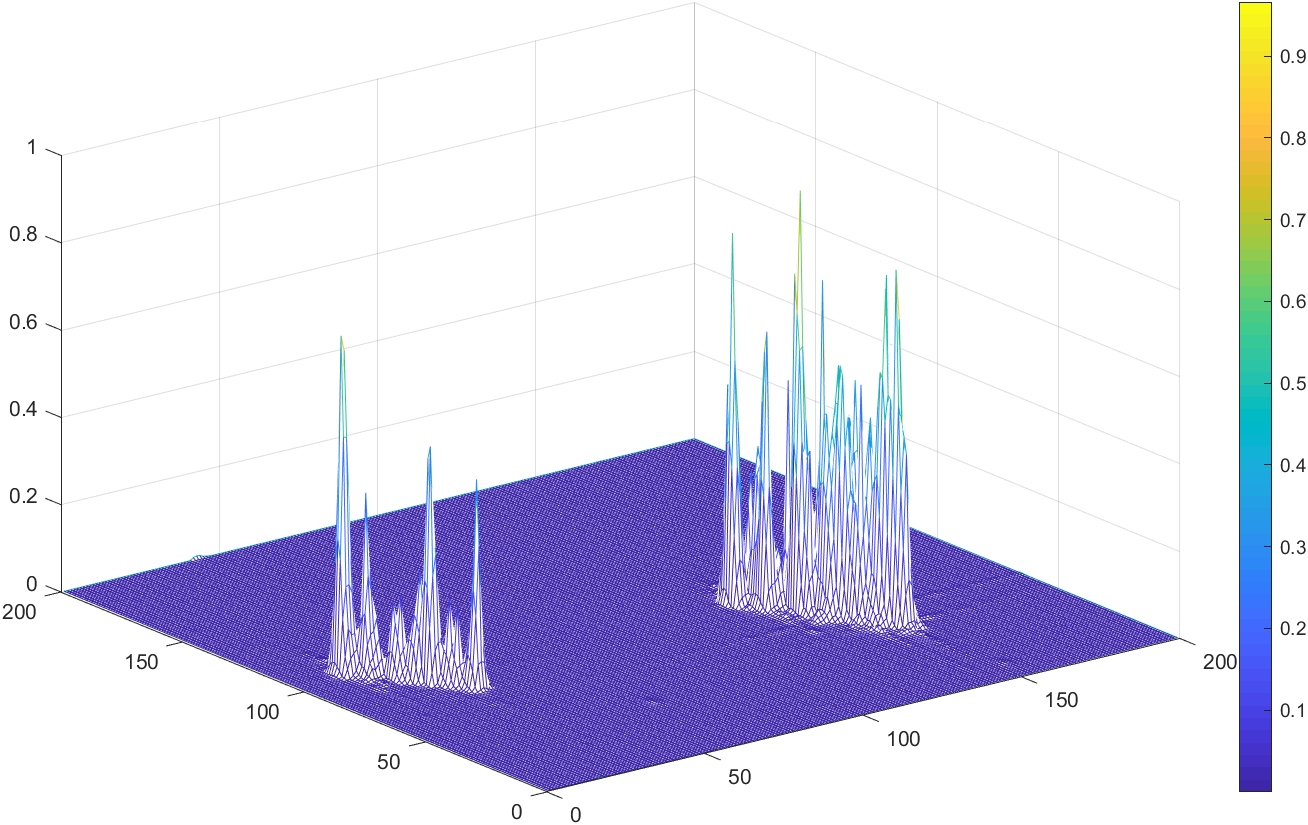
\includegraphics[width=9cm]{PCDMSPAN.png}}
    \subcaptionbox{SPAN图像\label{chap4:fig:subfig2}}
        {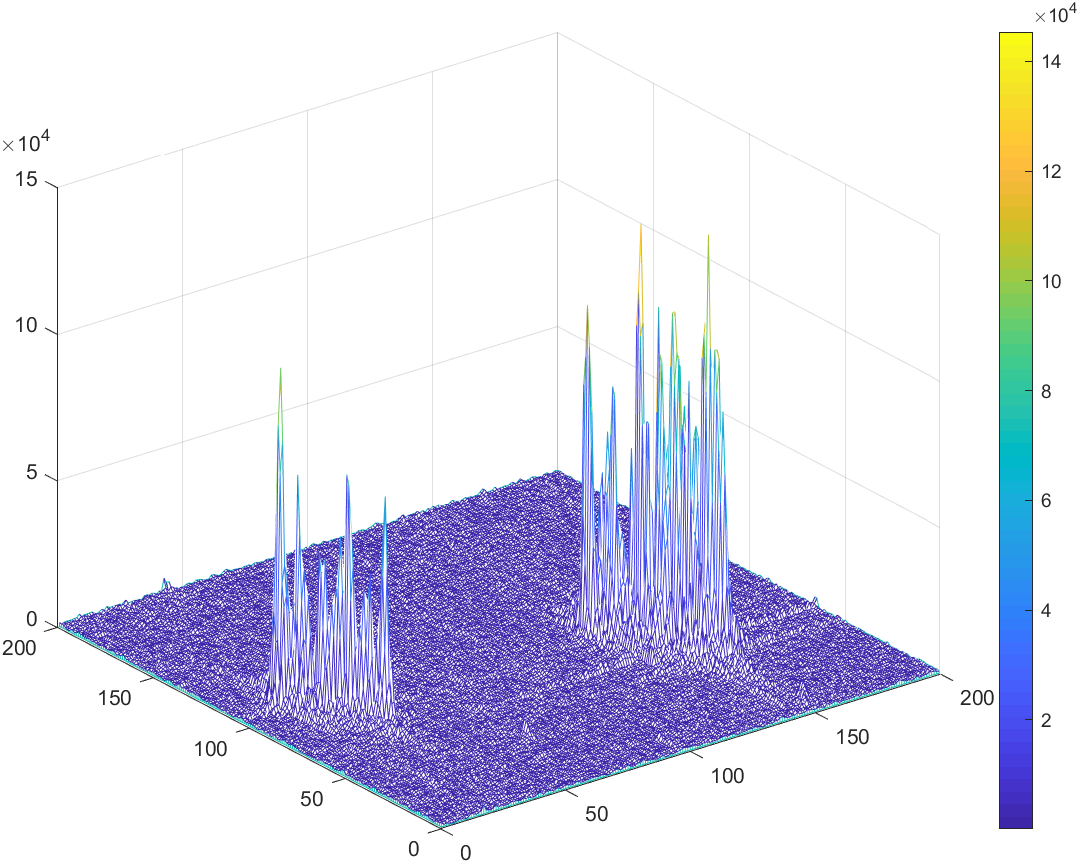
\includegraphics[width=9cm]{SPAN.png}}
    \caption{PCDNSPAN图像与SPAN图像对比}
    \label{fig:chap4:SPANCMP}
  \end{figure}

  图像检测结果,本次实验所使用的GPU为TiTAN V,运行显存内存为12G。基于MATLAB的串行算法运行的CPU为Intel(R) i7-9750H,系统内存为16G。
  为了验证检测结果的有效性,我们将PCDM方法与第二章实现的PWF方法进行对比如图\ref{fig:chap4:reultCMP}所示,从左到右依次为SPAN图像,PWF检测结果,PCDM检测结果。
  从检测结果上来看,PCDM得到的舰船检测结果与Pauli图像更加吻合,舰船边缘相较于PWF方法检测结果更加精确。算法的检测性能使用第二章定义的品质因数$F_1$来表示
  即正确检测数量与虚警数量和船只真实数量之和的比值。检测结果如表\ref{tab:chap4:detectresult}所示,PCDM的检测的品质因数高于PWF检测方法,可以得出结论PCDM算法对于
  复杂海况的适应能力比PWF强,即使面对不同海况依然可以保持高检测精度。

  在PCDM方法中不需要使用大量的海杂波像素去估计滤波器参数,该算法主要是计算大小为3x3的极化协方差差异矩阵及其特征值,因此算法在时间与空间性能上都优于极化白化滤波器方法。
  CPU串行与GPU并行的PCDM算法时间如表所示,因为GPU设备初始化开销代价所占比重较大,且CPU与GPU之间需要进行数据拷贝、通信与同步,所以本身在CPU上运行时间较短的程序在GPU上
  的加速比会降低。对于大小为1000x1000的SAR图像,经过多次实验测试,并行PCDM算法在Titan V上的运行的平均时间为0.69s,串行MATLAB方法在CPU上的运行时间为11.37秒,在时间性能上
  获得了近17倍的提升。

  
  \begin{figure}[h]
    \centering
    \subcaptionbox{SPAN图\label{chap4:fig:subfig2}}
        {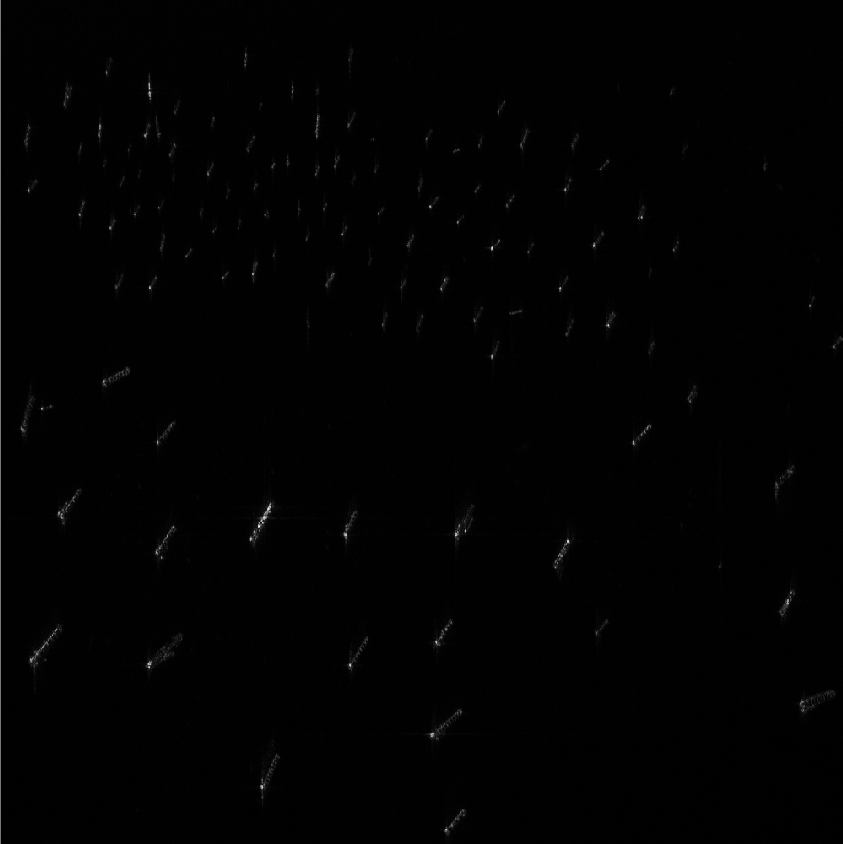
\includegraphics[width=7cm]{resultSPAN.png}}
    \subcaptionbox{PWF检测结果\label{chap4:fig:subfig2}}
        {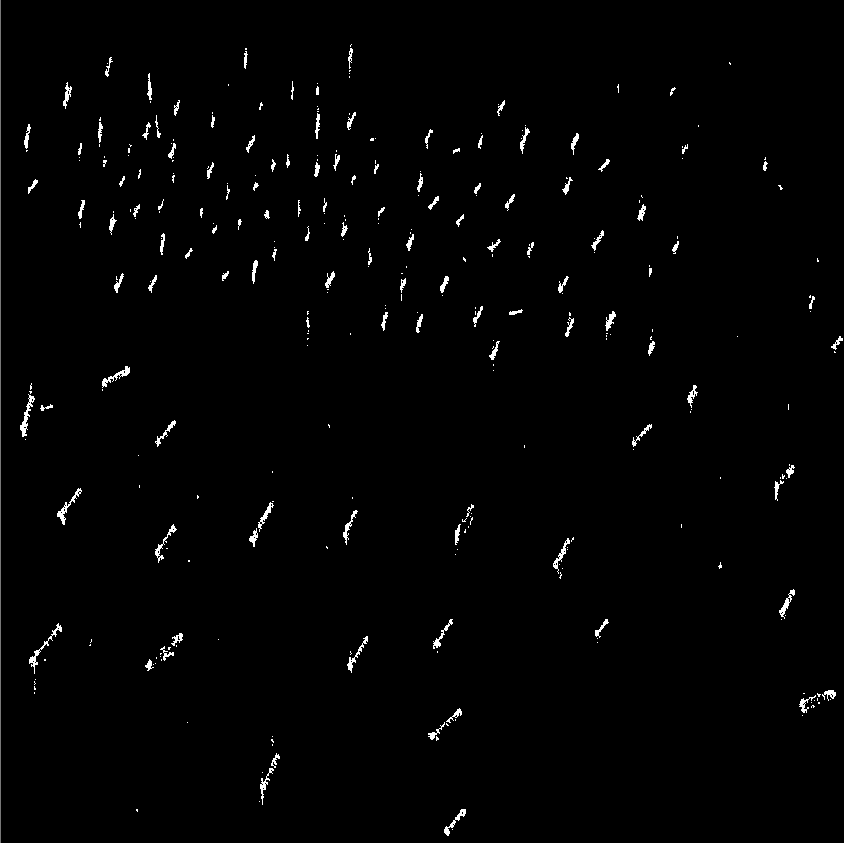
\includegraphics[width=7cm]{resultPWF.png}}

    \subcaptionbox{PCDM检测结果}
        {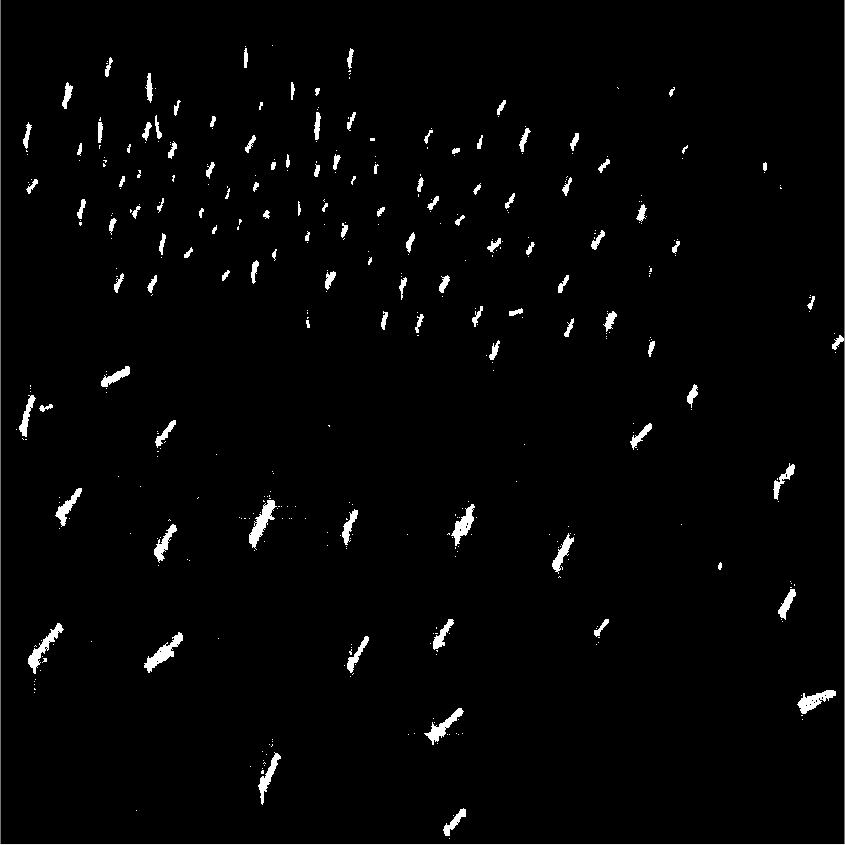
\includegraphics[width=7cm]{resultPCDM.png}}    
    \caption{舰船检测结果(a)SPAN图像;(b)PWF;(c)PCDM}
    \label{fig:chap4:reultCMP}
  \end{figure}

  \begin{table}[htb]
  \centering
    \begin{minipage}[t]{1\linewidth} % 如果想在表格中使用脚注,minipage是个不错的办法
    \caption[PCDM检测结果]{SAR图像检测结果对比}
    \label{tab:chap4:detectresult}
      \begin{tabularx}{\linewidth}{lXXXXXX}
        \toprule[1.5pt]
        {\heiti 检测方法} & {\heiti 船只数量} & {\heiti 总检测数量} & {\heiti 正确检测数量} & {\heiti 虚警数量} & {\heiti 漏报数量} & {\heiti $F_1$}\\ \midrule[1pt]
        PCDM & 118 & 120 & 117 & 3 & 1 & 0.967 \\
        PWF & 118 & 123 & 117 & 6 & 1 & 0.943 \\
        \bottomrule[1.5pt]
      \end{tabularx}
    \end{minipage}
\end{table}

  \begin{table}[htb]
  \centering
    \begin{minipage}[t]{1\linewidth} % 如果想在表格中使用脚注,minipage是个不错的办法
    \caption[PCDM算法运行时间对比]{不同平台算法运行时间对比}
    \label{tab:chap4:timeresult}
      \begin{tabularx}{\linewidth}{lXX}
        \toprule[1.5pt]
      {\heiti 检测算法} & {\heiti 运行平台} & {\heiti 运行时间/s} \\ \midrule[1pt]
        PCDM(MATLAB) & (Intel(R) i7-9750H CPU) & 11.4\\
        GPU并行PCDM & GPU(Titan V) & 0.67 \\
        PWF(C++) & (Intel(R) i9-7920X CPU) & 67.4\\
        GPU多线程PWF &  GPU(Titan V) & 2.1 \\
        多卡协同PWF & 2 GPU(Titan V) & 1.27 \\
        \bottomrule[1.5pt]
      \end{tabularx}
    \end{minipage}
\end{table}

\section{小结}
    对于极化SAR图像中的舰船目标检测,在本章我们实现了基于极化协方差差异矩阵的舰船检测方法。在该方法中,
    类比于光学图像检测中的LBP特征,我们引出了极化SAR图像的极化协方差差异矩阵(PCDM)的概念,PCDM矩阵计算了
    待检测像素与邻域像素的协方差矩阵差异,充分利用了空间相干信息,提高了舰船目标与背景杂波之间的对比度。
    接下来我们将PCDM矩阵应用于舰船检测,首先使用PCDM矩阵的SPAN值对船海像素做了一个粗略的划分,然后提取了PCDM矩阵
    的PSH极化特征,将该特征用于舰船目标检测,最后联合SPAN检测器得到的初步检测结果得到了最终的检测结果。实验结果
    表明PCDM方法可以有效的适应不同的复杂海况,相较于PWF算法,在检测精度、时间与空间消耗上都优于PWF算法。最后我们
    实现了基于GPU的并行PCDM方法,将图像像素对应的PCDM矩阵与PSH极化特征计算对应到每一个GPU线程中去并发执行。相比于
    串行执行的方式,并行的方法在时间性能上提升了近20倍,可以满足实时检测的要求


